\documentclass{beamer}
\setbeamertemplate{section in toc}[sections numbered]
\usefonttheme[onlymath]{serif}
\beamertemplatenavigationsymbolsempty
\setbeamertemplate{footline}{% 
  \hfill% 
  \usebeamercolor[gray!50]{page number in head/foot}% 
  \usebeamerfont{page number in head/foot}% 
  \insertframenumber\,/\,\inserttotalframenumber%
}
\usepackage{amsmath}
\usepackage{graphicx}
% \usepackage{caption}
% \usepackage[skip=0pt]{subcaption}
% \usepackage[tight,FIGTOPCAP]{subfigure}
\usepackage{lmodern}
\usepackage[round]{natbib}
% \usepackage{braket}
\usepackage{color}
\usepackage{bm}
\usepackage{amssymb}
\usepackage{bbold}
\usepackage{tikz}
\usepackage{empheq}
\usepackage{stackengine}
\usepackage{framed}
\usepackage[percent]{overpic}
\usepackage{adjustbox}
\usepackage{simpler-wick}
\usepackage{physics}
\DeclareMathOperator{\sgn}{sgn}
\tikzset{>=latex}
\newcommand{\blue}[1]{{\color{blue}{#1}}}
\newcommand{\md}{\mathrm{d}}
\newcommand{\ms}{\mathsf}
\newcommand{\bs}{\boldsymbol}
\newcommand{\mc}{\mathcal}
\renewcommand{\(}{\left(}
\renewcommand{\)}{\right)}
\renewcommand{\[}{\left[}
\renewcommand{\]}{\right]}

%Information to be included in the title page:
\title{Modeling Electronic Systems on Quantum Computers}
%\author{Apoorv Tiwar, Ammar Jahin, and Yuxuan Wang}
%\institute{University of Florida}
\date{University of Florida, October}

\begin{document}
\frame{\titlepage} 
\AtBeginSection[]
{
\begin{frame}
    \frametitle{Outline}
    \tableofcontents[currentsection]
\end{frame}
}

\begin{frame}
    \frametitle{Recap of last time}
    \begin{itemize}
        \item We discussed solving for the ground state $\ket{\Psi_0}$ and ground state energy of a molecule with $n$ electrons, \begin{align*}
            \hat{H} = \sum_{ij} h_1^{ij} a^\dagger_i a_j + \frac{1}{2} \sum_{ijkl} h_2^{ijkl} a^\dagger_i a^\dagger_j a_k a_l
        \end{align*}
        \item $a^\dagger_i$ creates a particle in the MO $\ket{\chi_i}$.
        \item For a calculations on a computer we need to to expand these orbital in some finite set of basis (AO). Let the number of basis be $m$.
        \item We use the occupation number representation \begin{align*}
            \ket{n_1, n_2, \dots, n_{m-1}, n_m}
        \end{align*}
        \item The Hilbert space dimensions is $\mc O(e^{n})$. 
        \item The Hartree-Fock approximation give us the state with the lowest energy that can also be written as a Slater determinant.   
    \end{itemize}
    

\end{frame}

% \begin{frame}
%     \frametitle{A word on entanglement}
%     For a bipartite system, we say that the two parts are entangled if measuring one part affect the other.
%     \begin{framed}
%         If we study a part of the system and ignore the rest, what is the (classical) uncertainty about the state of the studied part? 
%     \end{framed}
%     \begin{itemize}
%         \item Such uncertainty can be quantified by calculating the density matrix and tracing out the part of the system we don't want to study,  \begin{align*}
%             \rho_A = \Tr_{B} \rho_{AB}
%         \end{align*}
%         \item The trace sum over all degrees of freedom that belong to the subsystem B. 
%     \end{itemize}
    
%     We have to first decide how we are dividing our system up. 
% \end{frame}

% \begin{frame}
%     \frametitle{Entanglement}
%     \begin{columns}
%         \begin{column}[]{0.7\textwidth}
%             The question become tricky for a system of identical particles. Take again the case of the Hydrogen molecule. 
%         \end{column}
%         \begin{column}[]{0.3\textwidth}
%             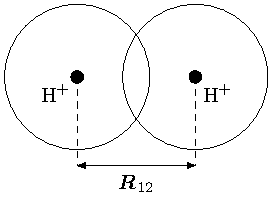
\includegraphics[scale = 0.7]{h2_ilust.pdf}
%         \end{column}
%     \end{columns}\pause
%     \underline{Is the state $\ket{\Phi_0} = a^\dagger_1 a^\dagger_2 \ket{0} = \ket{1100}$ entangled?}
%     \vspace{10pt}

%     Two ways we can think of to divide the system: 
%     \begin{enumerate}
%         \item Study one electron and ignore the other. 
%         \item Study one Hydrogen atom and ignore the other. 
%     \end{enumerate}
% \end{frame}

\begin{frame}
    \frametitle{Where quantum computer can help}
    \begin{columns}
        \begin{column}[]{0.5\textwidth}
            \begin{itemize}
                \item Classical computer can do HF efficiently.
                % \item In going beyond HF, the vastness of the Hilbert space the computer need to check make the computation less efficient.
                \item In going beyond HF the bottle necks are: \begin{enumerate}
                    \item Sampling the Hilbert space. 
                    \item Calculating the expectation value of the Hamiltonian.
                \end{enumerate}  
                \item A variational quantum eigensolver algorithm (VQE), put the exponentially hard part of the calculation on a quantum computer. 
            \end{itemize}
        \end{column}
        \begin{column}[]{0.5\textwidth}
            \begin{center}
                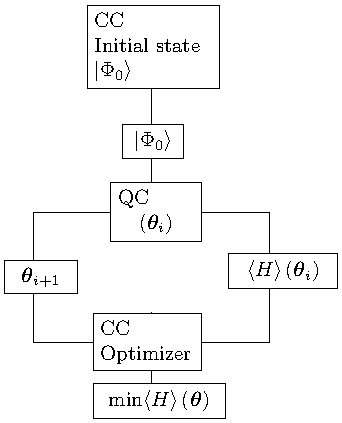
\includegraphics[scale=0.93]{VQE_flow_chart.pdf}
            \end{center}
        \end{column}
    \end{columns}
   
\end{frame}

\begin{frame}
    \frametitle{Outline}

    \tableofcontents

\end{frame}
\section{Introduction to circuit model for quantum computing}

\begin{frame}
    \frametitle{Qubits}
    A qubit lives in a 2 dimensional Hilbert space, $\mc H^1$. An arbitrary qubit state can be described as, 
    \begin{align*}
        \ket{\psi} = c_0 \ket{0} + c_1 \ket{1}.
    \end{align*}
    \pause
    A system of $N$ qubits lives in a $2^N$ dimensional Hilbert space, $\mc H^N$ such that, 
    \begin{align*}
        \mc H^N = \bigotimes_i^N \mc H^1_i
    \end{align*}
    An arbitrary state describing the system of $N$ qubits can be written as, 
    \begin{align*}
        \ket{\Psi} = \sum_{\{s_i\}} c_{1 \dots N} \ket{s_1 \dots s_N}, \ s_1, \dots s_N = \{0, \ 1\}
    \end{align*}

\end{frame}

\begin{frame}
    \frametitle{Gates}
    Operators can act on  one or two (or more) qubits independently. 
    \begin{itemize}
        \item These operators acting on the qubits are called quantum gates.
    \end{itemize}\pause
    \vspace{10pt}
    \begin{columns}
        \begin{column}[]{0.8\textwidth}
            Examples of 1-qubit gates: 
            \begin{itemize}
                \item The $X$-gate: $X\ket{0} = \ket{1}, \ X\ket{1} = \ket{0}$. 
                \item The $Z$-gate: $Z\ket{0} = \ket{0}, \ Z\ket{1} = -\ket{1}$.
                \item The $H$-gate: $H\ket{0} = \frac{1}{\sqrt{2}} \(\ket{0}  + \ket{1}\),\ H\ket{1}  = \frac{1}{\sqrt{2}} \(\ket{0} - \ket{1}\)$.       
            \end{itemize}
        \end{column}
        \begin{column}[]{0.2\textwidth}
            \centering
            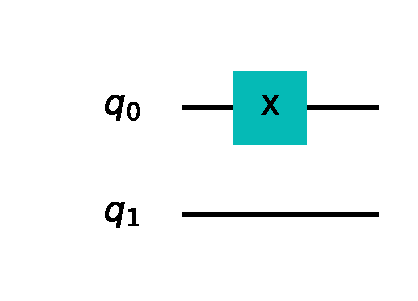
\includegraphics[scale=0.5, trim = 100 65 40 30, clip]{x_qubit_1.pdf} 
            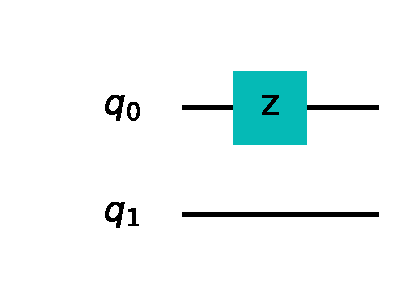
\includegraphics[scale=0.5, trim = 100 65 40 35, clip]{z_qubit_1.pdf} 
            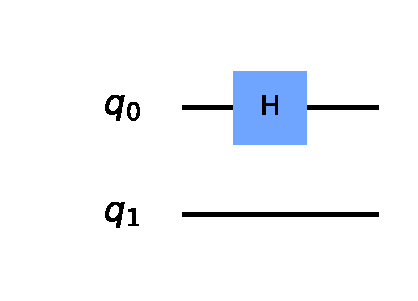
\includegraphics[scale=0.5, trim = 100 65 40 35, clip]{h_qubit_1.pdf} 
        \end{column}
    \end{columns}
    \pause
    \begin{columns}
        \begin{column}[]{0.8\textwidth}
            Example of 2-qubit gates: 
            \begin{itemize}
                \item Controlled-$X$ gate: $cX \ket{00} = \ket{00}, \ cX \ket{01} = \ket{01},
                cX \ket{10} = \ket{11}, \ cX \ket{11} = \ket{10}.$ It \emph{adds} the two qubits and puts the result in the second qubit
            \end{itemize}
        \end{column}
        \begin{column}[]{0.2\textwidth}
            \centering
            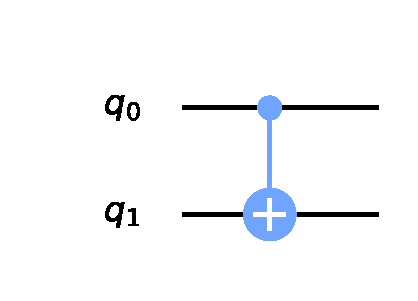
\includegraphics[scale=0.5, trim = 100 25 40 35, clip]{cx_qubit_2.pdf} 
        \end{column}
    \end{columns}
\end{frame}

\begin{frame}
    \frametitle{Circuits}
    Example 1:  $\ket{0} \rightarrow \ket{000},\ \ket{1} \rightarrow \ket{111} $. (Quantum repetition code.)
    \begin{center}
        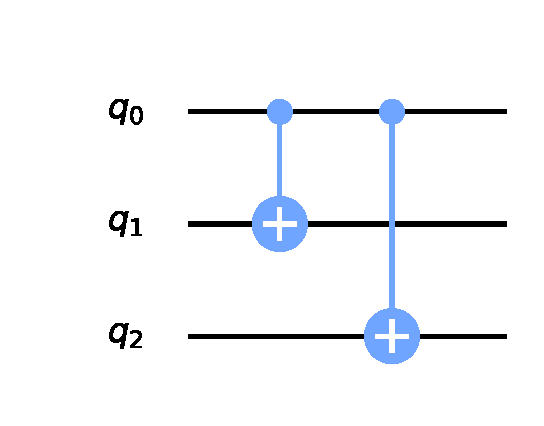
\includegraphics[scale = 0.5, trim = 30 25 40 35, clip]{repetition_circ.pdf}
    \end{center}
    \pause
    Example 2: $\ket{00} \rightarrow \frac{1}{\sqrt{2}}\(\ket{01} - \ket{10} \)$, (Adds entanglement.)
    \begin{center}
    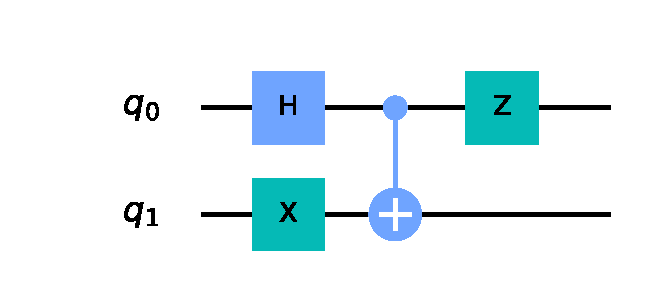
\includegraphics[scale = 0.5, trim = 30 25 40 35, clip]{add_ent.pdf}
    \end{center}
    \begin{itemize}
        \item The most prevalent model for quantum computations is the circuit model. 
        \item A circuit model is similar to how classical computers operate.
    \end{itemize}
\end{frame}


\section{Converting fermionic Hamiltonians to qubit Hamiltonians}
\subsection{Jordan-Wigner}
\begin{frame}
    \frametitle{Fermionic and qubit degrees of freedom} 
    % \begin{itemize}
    %     \item For $m$ orbitals, the Hilbert space is $2^{m}$ dimensional.
    %     \item A system of $m$ qubits is $2^{m}$ dimensional. 
    % \end{itemize}
    Fermionic system with $m$ orbitals: ($2^m$ dimensional) 
    \begin{align*}
        &\{a_i, a_j^\dagger\} = \delta_{ij}, \ \{a_i, a_j\} = 0. \\
        a^\dagger_i \ket{n_1 \dots n_i \dots n_m} &= \left\{ \begin{matrix}
            \zeta_i\ket{n_1 \dots n_i =1 \dots n_m},\  n_i = 0 \\ 
            \qquad \qquad \quad  0,\ \ \qquad  \qquad   n_i = 1
        \end{matrix} \right. \\ 
        & \zeta_i = (-1)^{\sum_{j=1}^{ i-1} n_j}\ \ \text{Parity counting}
    \end{align*}
    \pause
    Qubits system with $m$ qubits: 
    \begin{align*}
        &\qquad \qquad  \sigma^{+} = \frac{1}{2} (\sigma_x + i\sigma_y  ), \ \sigma^{-} = \frac{1}{2} (\sigma_x - i\sigma_y  ), \\ 
        &\qquad \qquad  \{\sigma^-_i, \sigma_j^{+}\} = 1, \ \{\sigma^-_i, \sigma_j^{-}\}=0, \ \  i = j , \\ 
        &\qquad \qquad  [\sigma^-_i, \sigma_j^{+}] = 0, \ \ [\sigma^-_i, \sigma_j^{-}] = 0, \ \  i \neq j \\ 
        &\sigma^{+}_i \ket{s_1 \dots s_i \dots s_m} = \left\{ \begin{matrix}
            \ket{n_1 \dots s_i = 1 \dots n_m}, && s_i = 0 \\ 
            0, && s_i = 1
        \end{matrix} \right.
    \end{align*}
\end{frame}

\begin{frame}
    \frametitle{Jordan-Wigner transformation}
    \begin{framed}
        We need a map from the fermionic operators the qubits operators.
    \end{framed}
    It seems reasonable to try, 
    \begin{align*}
        a^\dagger_i = \sigma_i^{+} , \ \  a_i = \sigma_i^{-}. 
    \end{align*}
    This doesn't produce the parity counting (the phase $\zeta_i$) that the fermionic operators generate when acting on basis states. 
    \pause
    Jordan-Wigner transformation: 
    \begin{align*}
        &\qquad \qquad \qquad \quad a^\dagger_i = \prod_{j = 1}^{i-1} \sigma^{z}_j \  \sigma_i^{+} \ \  a_i =  \prod_{j = 1}^{i-1} \sigma^{z}_j \  \sigma_i^{-}. \\
        &\prod_{j = 1}^{i-1} \sigma^{z}_j \  \sigma^{+}_i \ket{s_1 \dots s_i \dots s_m} = \left\{ \begin{matrix}
            \zeta_i \ket{n_1 \dots s_i = 1 \dots n_m}, && s_i = 0 \\ 
            0, && s_i = 1
        \end{matrix} \right.
    \end{align*}

\end{frame}

\begin{frame}
    \frametitle{Opertators transformation}
    \begin{center}
        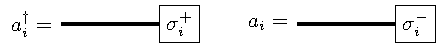
\includegraphics[]{jordan_wigner.pdf}
    \end{center}
    \pause
    \vspace{20pt}
    \begin{center}
        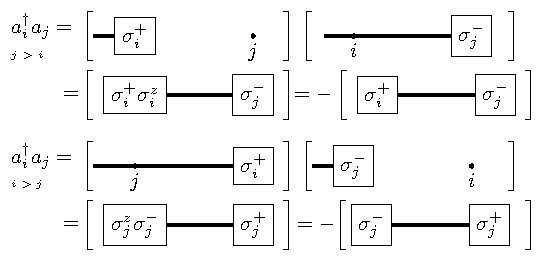
\includegraphics[scale = 1]{operator_jordan_wigner.pdf}
        % 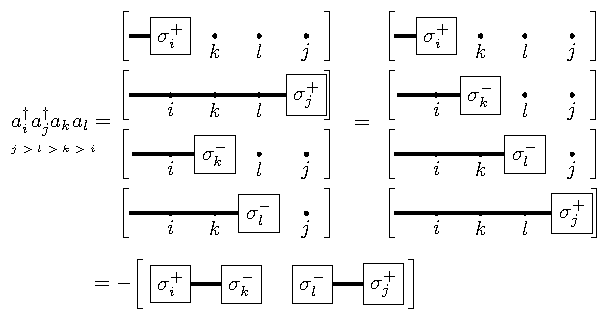
\includegraphics[scale = 0.71]{four_point_op_trans.pdf}
    \end{center}

\end{frame}


\begin{frame}
    \frametitle{Opertators transformation}

    \begin{center}
        % 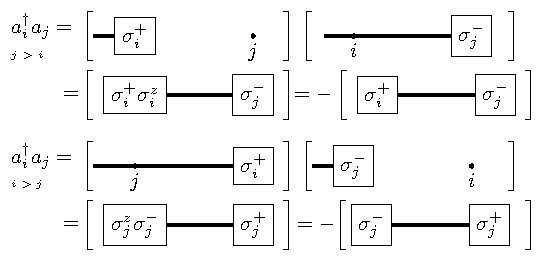
\includegraphics[scale = 1]{operator_jordan_wigner.pdf}

        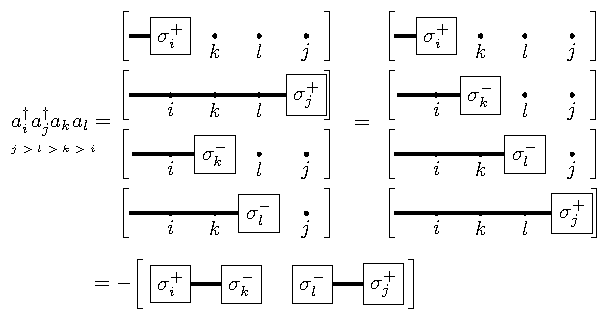
\includegraphics[scale = 1]{four_point_op_trans.pdf}
    \end{center}

\end{frame}

% \begin{frame}
%     \frametitle{Opertators transformation}
%     % Remember the fermionic Hamiltonian is, 
%     % \begin{align*}
%     %     \hat{H} = \sum_{ij} h^{ij}_1 a_i^\dagger a_j + \frac{1}{2} \sum_{ijkl} h_2^{ijkl} a_i^\dagger a_j^\dagger a_k a_j 
%     % \end{align*} 
%     \begin{columns}
%         \begin{column}[t]{0.6\textwidth}
%             \begin{align*}
%                 a_i^\dagger a_j =\left\{ \begin{matrix}
%                 \sigma_i^{+} \prod_{k = i}^{j-1} \sigma_k^{z} \  \sigma_j^{-}, &&  i < j \\ 
%                 \\
%                 - \sigma_i^{+} \prod_{k = i}^{j-1} \sigma_k^{z} \  \sigma_j^{-}, &&  i > j 
%             \end{matrix} \right. 
%             \end{align*}
            
%         \end{column}
%         \begin{column}[t]{0.4\textwidth}
%             If we order states on a line:
%             \\[8pt]
%             \centering
%             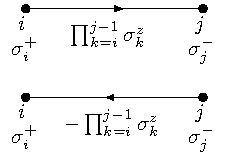
\includegraphics[]{ordering_fermi_1d.pdf}
%         \end{column}
%     \end{columns}
%     Note: State ordering is completely arbitrary. 
%     \begin{align*}
%         a^\dagger_i a^\dagger_j a_k a_l 
%     \end{align*}

% \end{frame}


\begin{frame}
    \frametitle{The qubit Hamiltonian}

    Remember the fermionic Hamiltonian is, 
    \begin{align*}
        \hat{H} = \sum_{ij} h^{ij}_1 a_i^\dagger a_j + \frac{1}{2} \sum_{ijkl} h_2^{ijkl} a_i^\dagger a_j^\dagger a_k a_j 
    \end{align*} 
    \begin{itemize}
        \item For our minimal model for the Hydrogen molecule we have $4$ basis, and hence the system will be represented by $4$ qubits. 
        \item After Jordan-Wigner transformation the uibit Hamiltonian will look something like this,
    \end{itemize}
     
    \begin{align*}
        \hat{H} = \sum_{i,j,k,l = 0}^ 3 j^{ijkl} \sigma^i_1 \sigma^j_2 \sigma^k_3 \sigma^l_4 
    \end{align*}
    To measure the $\expval*{\hat{H}}$, our quantum computer will need to measure $\expval*{\sigma^i_1 \sigma^j_2 \sigma^k_3 \sigma^l_4}$.
    \begin{itemize}
        \item There are other proposed maps. 
    \end{itemize}
\end{frame}

\begin{frame}
    \frametitle{Setting up the quantum circuit }
    For the Hydrogen example. 
    \begin{align*}
        \ket{\Phi_0} = \ket{1100}
    \end{align*}
    \begin{align*}
        a^\dagger_i a_i = \frac{1}{2} (1 + \sigma^z_i ). 
    \end{align*}
    
    \centering
    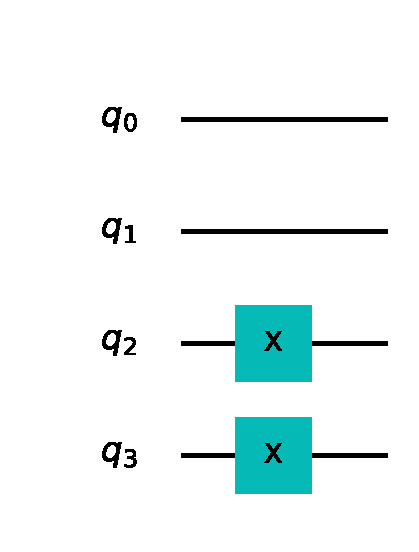
\includegraphics[scale=0.5]{initial_state_r.pdf}
\end{frame}


% \subsection{Parity and two-qubits reduction}


\section{VQE algorithms circuit designs for UCCSD}


\begin{frame}
    \frametitle{Unitary coupled-cluser (UCC) expansion}
    The UCC method uses the following ansatz, 
    \begin{columns}
        \begin{column}[]{0.55\textwidth}
            \begin{align*}
                &\ket{\Psi_0} = e^{T(\bm \theta) - T^\dagger (\bm \theta)} \ket{\Phi_0} \\ 
                &T(\bm \theta) = T_1(\bm \theta) + T_2(\bm \theta) + \dots \\ 
                & T_1(\bm \theta) = \sum_{\substack{m\in \text{emp} \\ i \in \text{occ}}} \theta^{mi} a^\dagger_m a_i \\ 
                &T_2(\bm \theta) = \frac{1}{2} \sum_{\substack{m, n\in \text{emp} \\ i, j \in \text{occ}}} \theta^{mnij} a^\dagger_m a^\dagger_n a_i a_j \\
                &  \quad \vdots
            \end{align*}
        \end{column}
        \begin{column}[b]{0.45\textwidth}
            \begin{align*}
                e^{T(\bm \theta) - T^\dagger (\bm \theta)} = e^{\sum_i \theta_i (\tau_i - \tau^\dagger_i)},
            \end{align*}
            where $\tau_i$ include all kinds of excitations. 
        \end{column}
    \end{columns}
   \pause
    \begin{itemize}
        \item For this ansatz to be computationally efficient we need to include only a few excitation operators. 
        \item UCCSD include single and double excitations.
        \item Next step would be to design a circuit that implement this unitary operation. 
    \end{itemize}
\end{frame}

\begin{frame}
    \frametitle{Trotterization}
    Different terms of $\tau_i$ don't necessarily commute which make simulating the exponential with quantum circuits not easy. 

    We make use of the following identity,
    \begin{align*}
        e^{\sum_i \theta_i (\tau_i - \tau^\dagger_i)} = \lim_{N \rightarrow \infty}\(\prod_i e^{\frac{\theta_i (\tau_i - \tau_i^\dagger)}{N}}\)^N
    \end{align*}
    \pause
    \begin{itemize}
        \item Taking $N$ to infinity is not possible for computations. Good results can be achieved by taking just a few trotter steps.
    \end{itemize}
    \begin{align*}
        e^{\sum_i \theta_i (\tau_i - \tau^\dagger_i)} = \(\prod_i e^{\frac{\theta_i (\tau_i - \tau_i^\dagger)}{\rho}}\)^\rho
    \end{align*}
    \begin{itemize}
        \item The smaller the $\theta_i$'s are the better the approximation.
        \item It's better to start with a good initial guess. 
    \end{itemize}
    
\end{frame}

\begin{frame}
    \frametitle{Converting to qubits operations}
    \framesubtitle{one-body exponentials}

    One body exponential $e^{\theta (a^\dagger_m a_i - a^\dagger_i a_m )}$. Note: $m>i.$ 
    \begin{align*}
        &a^\dagger_m a_i - a^\dagger_i a_m = -\sigma^{-}_i \(\prod_{s=i+1}^{m-1} \sigma_s^z\) \sigma^{+}_m  + \sigma^{+}_i  \(\prod_{s=i+1}^{m-1} \sigma_s^z\) \sigma^{-}_m \\
        % &\sigma^{+} \sigma^{z} = -(\sigma^{-} \sigma^{z})^\dagger = - \sigma^{+} \\ 
        &a^\dagger_m a_i - a^\dagger_i a_m = \frac{i}{2} \[ \sigma^{y}_i \(\prod_{s=i+1}^{m-1} \sigma_s^z\) \sigma^{x}_m  - \sigma^{x}_i \(\prod_{s=i+1}^{m-1} \sigma_s^z\) \sigma^{y}_m \]
    \end{align*}
    Note that the two terms commute. 
    \pause

    We rotate $\sigma^x$ and $\sigma^y$ to $\sigma^{z}$,
    \begin{align*}
        e^{i\theta \sigma^{y}_i \(\prod_{s=i+1}^{m-1} \sigma_s^z\) \sigma^{x}_m}  = H_m R^x_i(\pi/2)\(e^{i\theta \sigma^{z}_i \(\prod_{s=i+1}^{m} \sigma_s^z\) } \)H^\dagger_m R^{x\dagger}_i(\pi/2), 
    \end{align*}
    using,
    \begin{gather*}
        H \sigma_z H^\dagger  = \sigma_x \\ 
        R^x\(\pi/2\) \sigma_z R^{x\dagger}\(\pi/2\)  = \sigma_y 
    \end{gather*}
\end{frame}

\begin{frame}
    \frametitle{Converting to qubit operations}
    \framesubtitle{one-body exponentials}
    Need to implement $\exp\[i\theta \sigma^{z}_i \(\prod_{s=i+1}^{m} \sigma_s^z\) \]$. 
    \begin{itemize}
        \item $\prod_{s=i+1}^{m} \sigma_s^z$ counts the parity between qubits $i$ and $m$. The answer is plus or minus. 
        \item $e^{\pm i \theta\sigma^z_i }$ makes a rotation around the $z$-axis on the $i$-th qubit accordingly. 
    \end{itemize}
    \pause
    Example: $\exp\[i\theta \sigma^{y}_1 (\sigma_2^z \sigma_3^z )\sigma^{x}_4 \]$ for Hydrogen molecule.  
    \begin{center}
        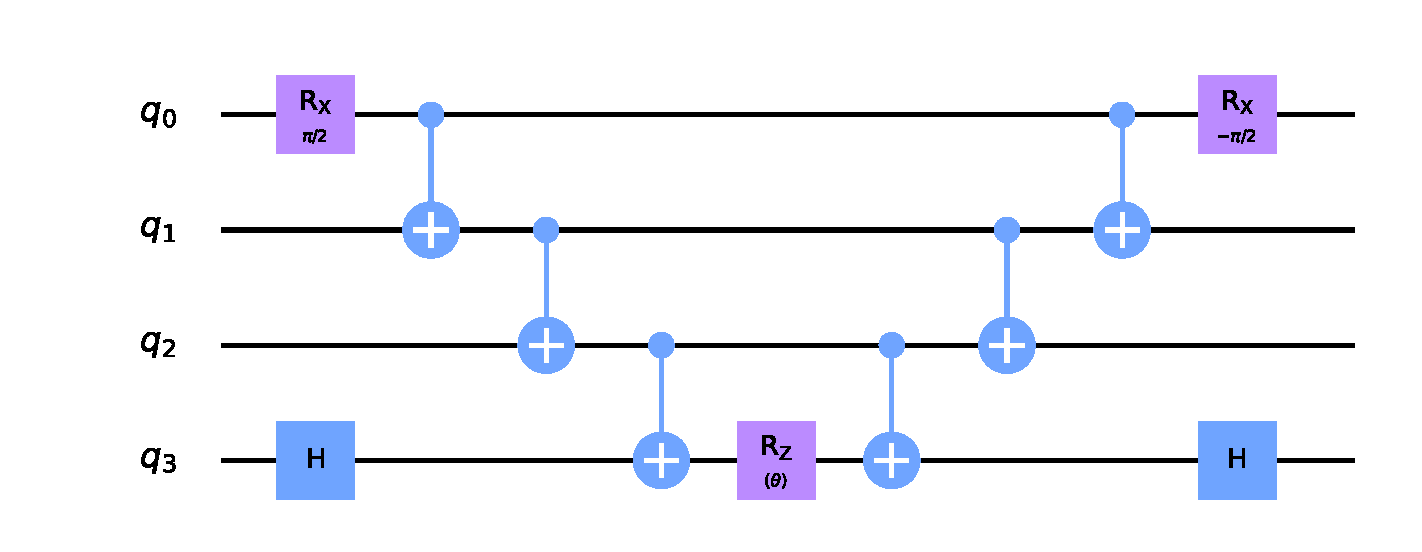
\includegraphics[scale = 0.45, trim = 65 0 0 0 , clip]{a_4a_1_r.pdf} 
    \end{center}
\end{frame}

\begin{frame}
    \frametitle{Converting to qubit operations}
    \framesubtitle{two-body exponentials}

    Two-body exponential $e^{\theta (a^\dagger_m a^\dagger_n a_j a_i - a^\dagger_i a^\dagger_j a_n a_m  )}$, and assume $j>i$, and $m>n$ 

    \begin{align*}
        a^\dagger_m a^\dagger_n a_i a_j - a^\dagger_i a^\dagger_j a_n a_m  = &\sigma^{-}_i \(\prod \sigma^{z}\) \sigma^{-}_j\  \sigma^{+}_n \(\prod \sigma^{z}\) \sigma^{+}_m \\ 
        - & \sigma^{+}_i \(\prod \sigma^{z}\) \sigma^{+}_j\  \sigma^{-}_n \(\prod \sigma^{z}\) \sigma^{-}_m \\ 
        = & \frac{i}{4} \sigma^{x}_i \(\prod \sigma^{z}\) \sigma^{x}_j \  \sigma^{x}_n \(\prod \sigma^{z}\) \sigma^{y}_m \\ 
        + &\text{terms with odd } \sigma^{y} 
    \end{align*}
    This generate $8$ terms, all of which will commute. As before we rotate $\sigma^x$ and $\sigma^y$ to $\sigma^{z}$, 
    \begin{align*}
        H_i H_i H_n Y_m e^{\frac{i\theta}{4} \(\sigma^{z}_i \(\prod_{i+1}^{j} \sigma^{z}\)\  \(\prod_{n}^m \sigma^{z}\) \)} H^\dagger_i H^\dagger_i H^\dagger_n Y^\dagger_m
    \end{align*}
    
\end{frame}

\begin{frame}
    \frametitle{Converting to qubit operations}
    \framesubtitle{two-body exponentials}
    Note we only add parity from $m$ to $n$ and from $j$ to $i+1$ then perform the rotation on the $i$-th qubit.
     
    Example: $\exp{\[ i\theta \sigma^x_1 \sigma^x_2 \sigma^x_3 \sigma^y_4  \ \]}$ for the Hydrogen molecule, 

    \begin{center}
        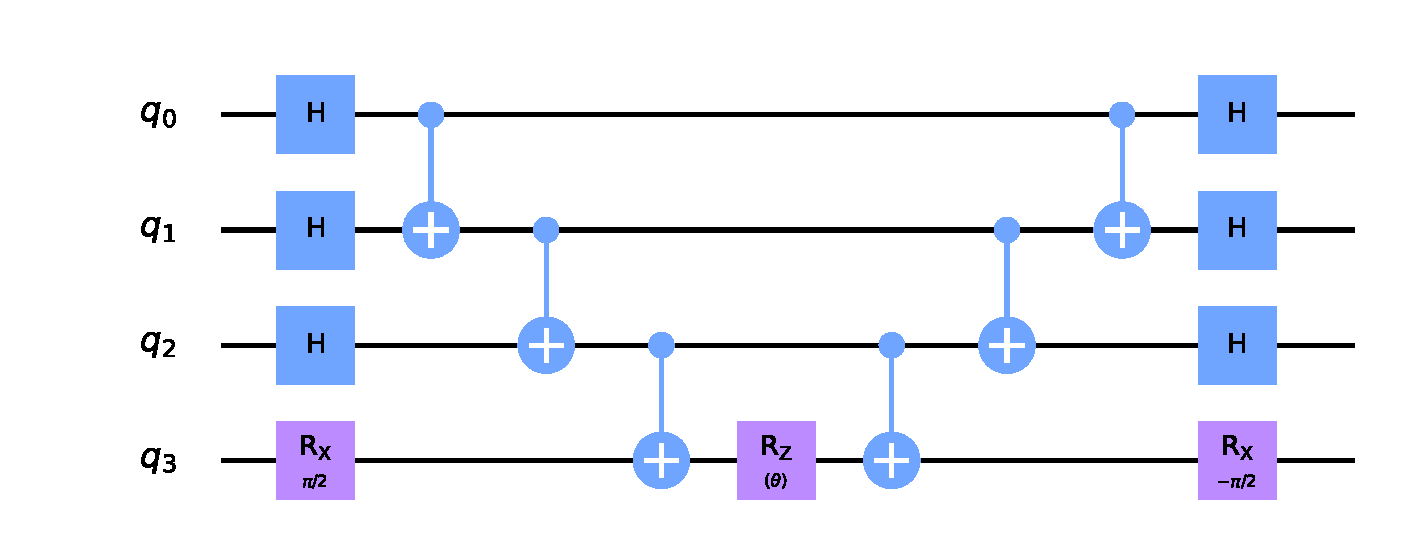
\includegraphics[scale=0.45, trim = 65 0 0 0 , clip]{a1a2a3a4_r.pdf}
    \end{center}
\end{frame}

\begin{frame}
    \frametitle{Measuerment}
    The Hamiltonian expectation value is written as, 
    \begin{align*}
        \ev*{\hat{H}} = \sum_{i,j,k,l = 0}^ 3 j^{ijkl}\ev*{\sigma^i_1 \sigma^j_2 \sigma^k_3 \sigma^l_4} 
    \end{align*}
    The computational basis is the $z$-axis. To measure the expectation value a general string of Pauli operators, we need a post-rotation circuit. 
    \begin{itemize}
        \item Measuring the qubits gives a string of $0$'s and $1$'s, $\{s_i\}$.
        \item $P(\{ s_i \}) = |\braket{\{s_i\}}{\Psi_0}|^2$
        \item To measure the $i$-th qubit with respect to the $x$ or $y$-axes we need to rotate our basis for the $i$-th qubit using $H_i$ or $R_i^{x}(\pi/2)$ respectively. 
        \item Any Pauli string has eigenvalues of either $\pm 1$.
        \item $\ev*{\sigma^i_1 \sigma^j_2 \sigma^k_3 \sigma^l_4} = P(1) - P(-1)$ 
    \end{itemize}
\end{frame}

\begin{frame}
    \frametitle{}
    The end result look something like this: 
    \begin{center}
        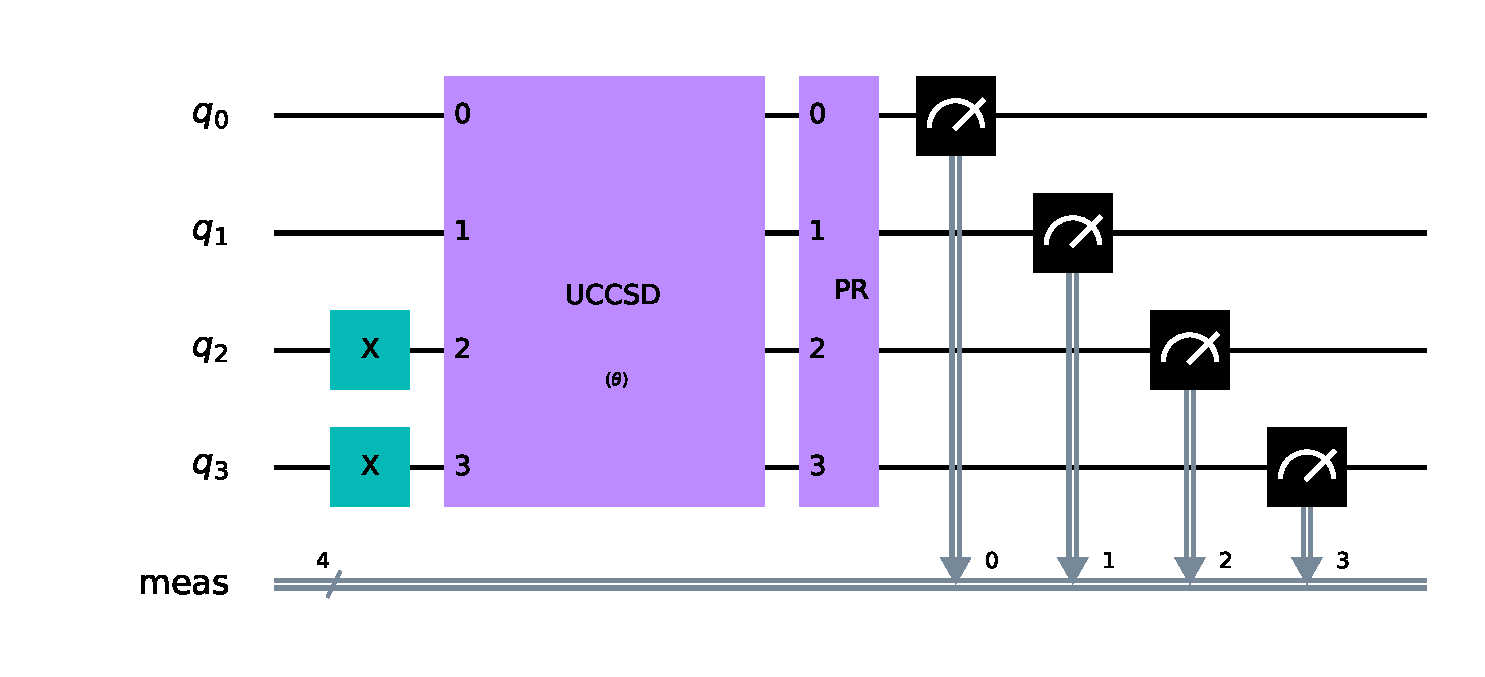
\includegraphics[scale=0.445, trim = 65 0 0 0 , clip]{uccsd_qc.pdf}
    \end{center}
    \begin{columns}
        \begin{column}[]{0.7\textwidth}
            \begin{enumerate}
                \item Initialize the qubits 
                \item Apply the UCCSD gate with parameters $\bm \theta$
                \item Apply post-rotations .
                \item Measure the qubits.
            \end{enumerate}
        \end{column}
        \begin{column}[]{0.3\textwidth}
            \begin{align*}
                &\text{Comparison:}\\
                &E_{\text{HF}} = -1.116\\
                &E_{\text{UCCSD}} = -1.137 \\ 
                &E_{exact} = -1.166
            \end{align*}
        \end{column}
    \end{columns}
\end{frame}

\begin{frame}
    \frametitle{Summary}

    The VQE method can be summarized as follows: 
    \begin{columns}
        \begin{column}[]{0.5\textwidth}
            \begin{enumerate}
                \item A classical computer calculate the Hamiltonian and come up with an initial state. 
                \item A quantum computer samples the Hilber space and measure the energy. 
                \item A classical computer will run an optimization routine to minimize the energy expectation value. 
            \end{enumerate}
        \end{column}
        \begin{column}[]{0.5\textwidth}
            \begin{center}
                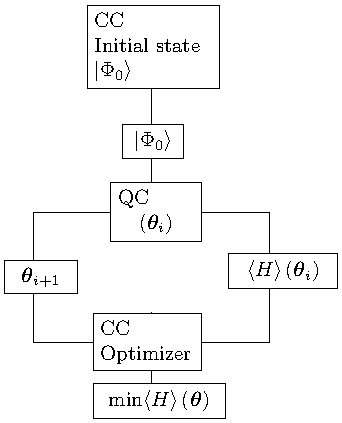
\includegraphics[scale=0.93]{VQE_flow_chart.pdf}
            \end{center}
        \end{column}
    \end{columns}
    

\end{frame}

\end{document} 